\documentclass[pdf]{note}
\usepackage[usenames,dvipsnames]{color}     % for color coding during editing
\usepackage{verbatim}
\usepackage{url}
\usepackage[latin1]{inputenc}
\usepackage[T1]{fontenc}
\usepackage{ae}
\usepackage{amsmath, amssymb}
\usepackage{subfigure}
\usepackage{xspace}
\usepackage{multicol}

%\usepackage{finesse}
%\newcommand{\Finesse}{\textsc{Finesse}\xspace}

\usepackage{fancyvrb}
\DefineVerbatimEnvironment{finesse}{Verbatim}
{formatcom=\small}

\author{Charlotte Bond}
\shorttitle{Wave front reconstruction using fast Fourier transforms}
\title{Wave front reconstruction using fast Fourier transforms}
\date{\today}
\issue{1}

%\usepackage{float}
%\usepackage{parskip}
%\usepackage{xspace}
\usepackage[pdftex,a4paper,pagebackref=true,pdfpagelabels=true]{hyperref}
\definecolor{linkcolor}{rgb}{.8,0,0}
\definecolor{urlcolor}{rgb}{0,0,.7}
\definecolor{citecolor}{rgb}{0,.5,0}
\definecolor{acrocolor}{rgb}{0,0,.7}
\hypersetup{bookmarksopen,colorlinks=true}
\hypersetup{pdfstartview=FitH}
\hypersetup{linktocpage=true,bookmarksnumbered=true}
\hypersetup{plainpages=false,breaklinks=true}
\hypersetup{linkcolor=linkcolor,citecolor=citecolor,urlcolor=urlcolor}

\newcommand{\tcr}{\textcolor{red}}

\let \IG \includegraphics

\begin{document}
\maketitle
\tableofcontents
\vspace{1cm}\hrule \vspace{1cm}

\section{Introduction}
In theory a wave front reconstruction technique in the Fourier domain, for
a Shack-Hartmann WFS, can provide an anti-aliasing Wiener filter (Correia 2014).
In this note the analysis using a numerical approach/simulations are presented and
compared with the theoretical results. 


\section{Fourier transform of the wavefront}

Firstly we look at the phase directly and compare an analytic PSD (power spectral density) 
with that using a numerical analysis and Fast Fourier Transforms (FFTs).
Phase screens are generated using OOMAO functions which use
the analytical equation for the PSD:
\begin{equation}
W_{\phi} = 0.49 \ r_0^{-5/3} \left((2\pi)^2 \left(f_x^2+f_y^2+\frac{1}{L_0^2}\right)\right)^{-11/6}
\end{equation}
where $k_{x/y}$ are the spatial frequencies in $x$ and$y$, $r_0$ is the Fried parameter
and $L_0$ is the outer scale.
To get a realisation of the phase random noise is added to $\sqrt{W_{\phi}}$ and
the inverse Fourier Transform is used to convert to the spatial domain.

The power spectral density can be calculated from the Fourier transform:
\begin{equation}
\mathrm{PSD}(\phi(x,y)) = < \left| \mathcal{F} (\phi(x,y))\right|^2 >
\end{equation}
where we average over different realisations of the phase (a \emph{cube} of phase)
to average out the noise.

In the case of numerical calculations of the Fourier transform care should be
taken with the units.  In this case, using the standard Matlab FFT we have an
individual PSD (in 2D) as:
\begin{equation}
PSD = \frac{|FFT(w(x,y)\phi(x,y))|^2}{S_2 f_s^2} 
\end{equation}
where $f_s$ is the sampling frequency, $w(x,y)$ is a possible weighting function
and $S_2$ is a normalisation constant given by:
\begin{equation}
S_2 = \sum_{i=0}^N \sum_{j=0}^N w_{i,j}^2
\end{equation}
In the case where no window is used we have $S_2 = N^2$, the number of
points in the grid.

\subsection{Example parameters}

In this example I use a grid of $200\times 200$ pixels, with dimensions of the telescope
diameter, 8\,m.  This gives a sampling frequency of $f_s = 25$\,m$^{-1}$.
To characterise the phase distortion we need the atmosphere parameters $r_0 = 15$\,cm
and $L_0 = 30$\,m.  Using OOMAO a cube of phase screens is produced.  The functions
were also modified to produce one full phase map, one containing just the low
order spatial frequencies and one containing only the high order spatial frequencies.
The cut off between the two is determined by the number of lenslets we will use
in later examples, $20\times20$.  The 3 different phase screens are illustrated
in figure~\ref{fig:phase_screens}, for different random realisations of the phase.

\begin{figure}[htbp]
    \centerline{
      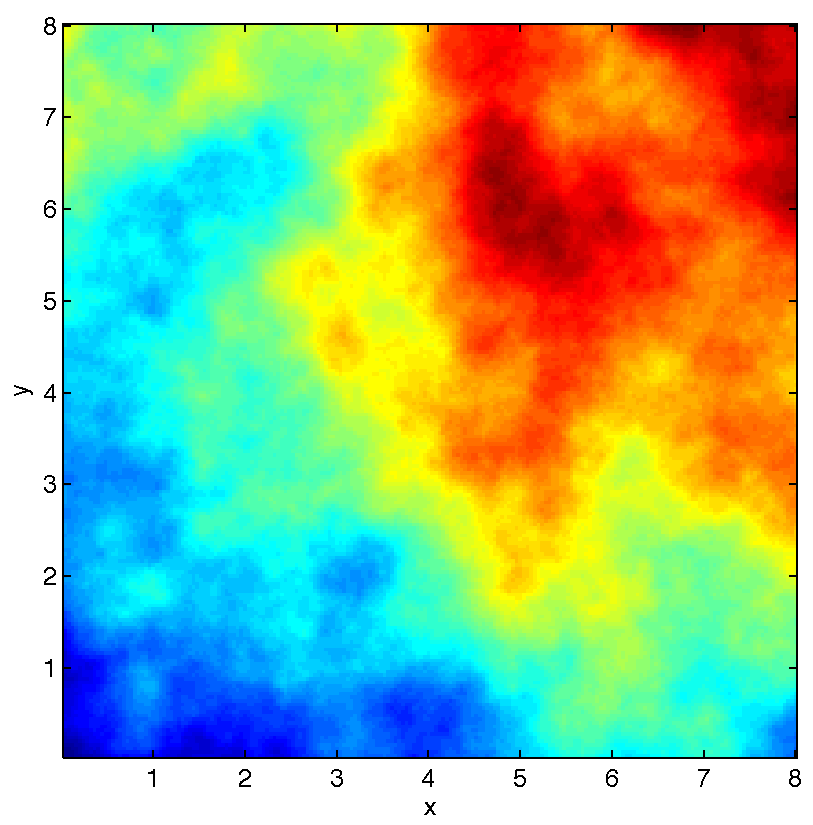
\includegraphics[scale=.4]{plots/total_phase}
      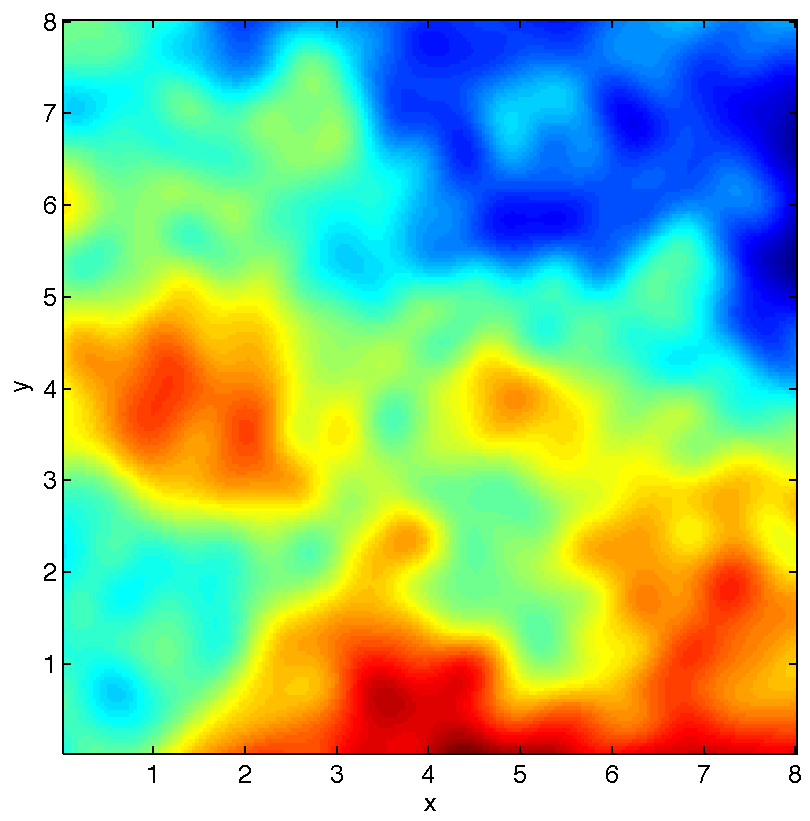
\includegraphics[scale=.4]{plots/LO_phase}
      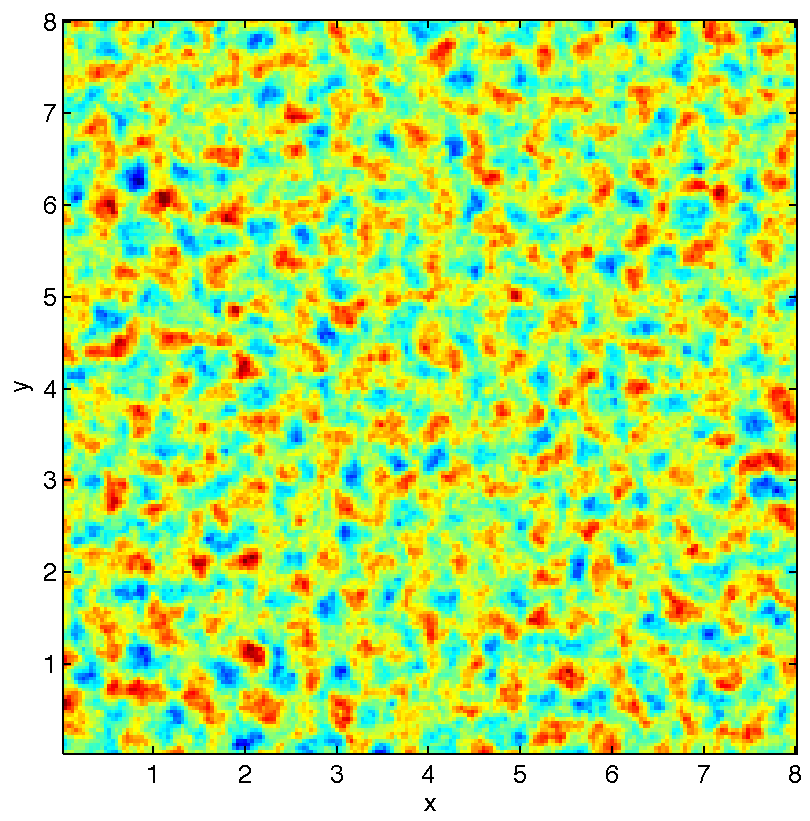
\includegraphics[scale=.4]{plots/HO_phase}
    }
    \caption{3 different phase screens produce in OOMAO.  Left: includes all
    	spatial frequencies up to that defined by the sampling of the grid.  Centre:
	includes only low spatial frequencies up to a limit defined by the sub-aperture
	spacing.  Right: contains only high spatial frequencies above that defined by the
	sub-aperture spacing.
    }
    \label{fig:phase_screens}
\end{figure}



\begin{figure}[htbp]
    \centerline{
      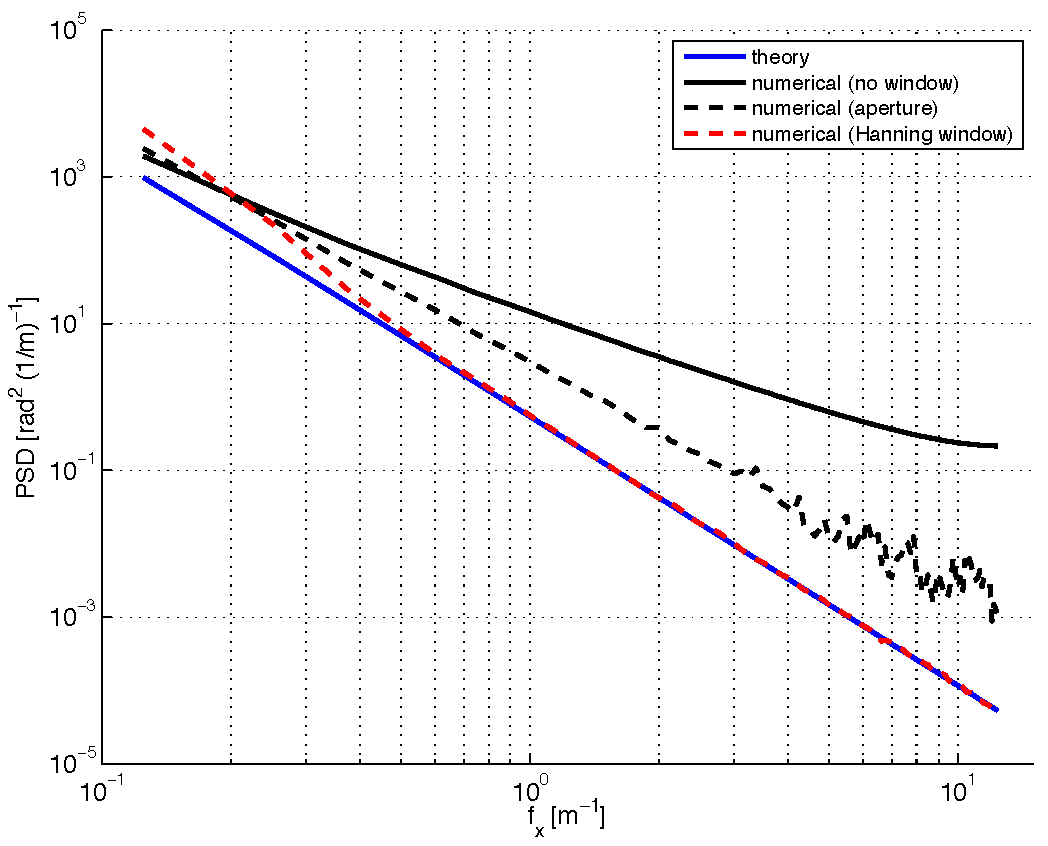
\includegraphics[scale=.6]{plots/phase_PSDs1}
    }
    \caption{Power spectral density of the phase, calculated analytically and numerically
    	using different windowing functions.  The Hanning window gives the closest match to
	the analytics.
    }
    \label{fig:phasePSD1}
\end{figure}

Questions:
- why is the Hanning window over-estimating low freqs?
- Why is the aperture case so noisy at high freqs?
- why isn't the no window case better?  Where does the discrepancy come from?  Sharp cut offs
at the edge? 



\begin{figure}[htbp]
    \centerline{
      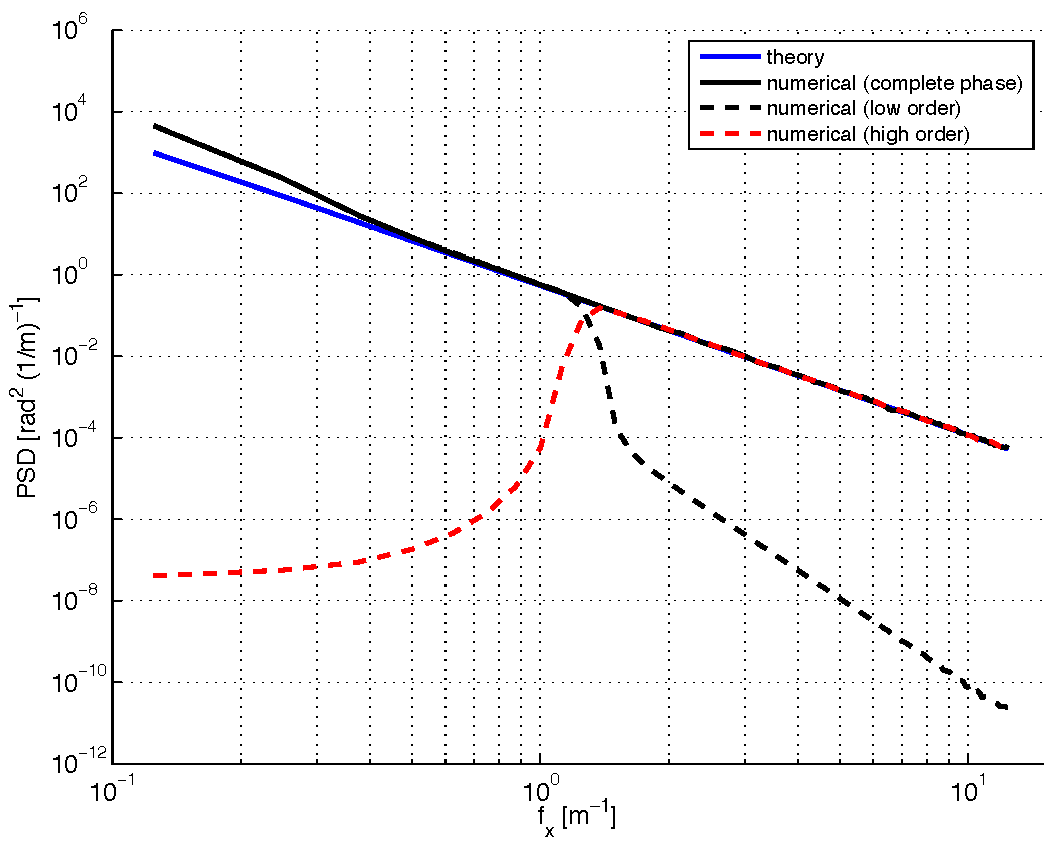
\includegraphics[scale=.6]{plots/phase_PSDs2}
    }
    \caption{Power spectral densities of the phase.  The analytical result is shown
    		as well as the numerical calculation for 3 phase types: the complete phase,
		including all spatial frequencies as detectable for a given sampling; the low
		order phase including only low spatial frequencies (below the Nyquist frequency
		set by the lenslet seperation); and high order phase including only the spatial
		frequencies above this Nyquist frequency.
    }
    \label{fig:phasePSD2}
\end{figure}


add in 2D plots, residuals?

\section{Fourier transform of the slopes}

Now we consider the Fourier transform of the slopes produced by a Shack Hartmann
WFS and again compare with the analytic expression.

%Different cases:
%1) fully illuminated SH -> square grid and no weighting/ weighting
%2) telescope aperture applied -> use weightings/no weightings.  Adding in the aperture, does it
%cause significant difference between numerical and theory.









\end{document}


